\documentclass{article}
\usepackage[utf8]{inputenc}
\usepackage[english]{babel}
\usepackage{libertine}
\usepackage[a4paper]{geometry}
\usepackage{parskip}
\usepackage{booktabs}
\usepackage{tabularx}
\usepackage{enumitem}
\usepackage{graphicx}
\usepackage[dvipsnames]{xcolor}
\usepackage{float}
\usepackage{wrapfig}
\usepackage{multicol}
\usepackage{multirow}
\usepackage{vwcol}
\usepackage{dashrule}
\usepackage{pdfpages}
\usepackage[bottom,hang]{footmisc}
\usepackage{setspace}
\usepackage{siunitx}
\usepackage[official]{eurosym}

\setlength{\footnotemargin}{2mm}
\setlength{\footnotesep}{2mm}

\usepackage{chngcntr}
\counterwithin{figure}{section}

\usepackage{blindtext}

\usepackage{csquotes}
\MakeOuterQuote{"}

\usepackage{hyperref}
\hypersetup{
	pdftitle={Unofficial Guide to the Conversion of Singapore Driving Licence -- Munich},
	pdfauthor={Sun Yudong},
	bookmarksnumbered=true,
	bookmarksopen=true,
	bookmarksopenlevel=2,
	pdfstartview=Fit,
	pdfpagemode=UseOutlines,
	colorlinks=true,
	linkcolor=black,
	filecolor=magenta,      
	urlcolor=blue
}
\urlstyle{same}

\graphicspath{{attachments/}}

% Self declared
\newcommand{\blanko}[0]{\textcolor{white}{.}}
\newcommand{\datum}[0]{\today}
\newcommand{\de}[1]{\textcolor{NavyBlue}{\textit{#1}}}
\newcommand{\cost}[1]{\textbf{Cost}\hspace{1cm}\SI[round-precision=2,round-mode=places,round-integer-to-decimal]{#1}[]{}~\euro}
\newcommand{\impt}[1]{\textcolor{Maroon}{#1}}
% / Self declared


\usepackage{fancyhdr}
% Meant to be distributed digitally

\pagestyle{fancy}
\fancyhf{}
\fancyhead[L]{Conversion of Singapore Driving Licence}
\fancyhead[R]{Stand: \datum}
\cfoot{\thepage}

\title{\vspace{-1cm}{\large Unofficial Guide}\\Conversion of Singapore Driving Licence \\ {\large Landeshauptstadt München}}
\author{Sun Yudong}
\date{{\normalsize caa.} \datum}

\begin{document}

\maketitle

\section{Introduction}
    According to the BMVI\footnote{\scriptsize \url{www.bmvi.de/SharedDocs/DE/Artikel/StV/Strassenverkehr/gueltigkeit-auslaendischer-fahrerlaubnisse-in-deutschland.html}} Foreigners from non EU/EEC countries can drive for 6 months with their foreign driving licence after they enter Germany and register their address with the authorities (\de{Anmeldung}). Should you wish to drive beyond that, you will have to convert your licence.\footnote{The author is unfortunately not sure as to whether going back to Singapore and coming back practically (not legally) restarts the 6 months.}
    
    To convert your licence, the laws differ from state to state. This document is mainly to document the process the author went through to convert their driving licence here in Munich and serve as an English guide for other Singaporeans coming over to Munich. 
    
    It is recommended to go through the whole document to get an overview first. The process is relatively straightforward, just a lot of waiting.
    
        \subsection{Prerequisites}
        \begin{enumerate}
            \item You are here on a long term visa (e.g. Work, Study, etc.)
            \item You have done your \de{Anmeldung} and registered your address with the authorities. Your registered address in under the administration of \de{Kreisverwaltungsreferat München}. 
            \item You have a valid passport. A Residence Permit or \de{Aufenthaltstitel} is a good-to-have but not necessary at this stage. 
            \item You have a valid \impt{\textit{physical}} Singaporean Qualified Driving Licence (QDL).
        \end{enumerate}
        
        \subsection{Key Numbers}
        \begin{center}
            \renewcommand{\arraystretch}{1.2}
            \begin{tabular}{@{}ll@{}}
                \toprule
                Advertised & 3 - 4 Weeks \\
                Actual (Author) & 10 - 12 Weeks\footnotemark\\
                \bottomrule
            \end{tabular}
        \end{center}
        \footnotetext{This was a result of the \de{Fahrerlaubnisbehörde} driving license authority not ordering my licence after the police has verified its legitimacy, elaborated in Section \ref{subsec:roadblocks}}
        
        \vspace{\parskip}
        
        We give them the benefit of the doubt as they did indicate that the validation of the licence will take 3-4 weeks, making a total of 6-8 weeks.

\newpage
\tableofcontents
\newpage

\section{Translation of Licence}
    \cost{55}
    
    Unfortunately, the translation provided by the Automobile Association in Singapore through the International Driving Permit is \textbf{not accepted} as a valid translation of the licence. You will need the following document instead:

    \begin{figure}[H]
        \centering
        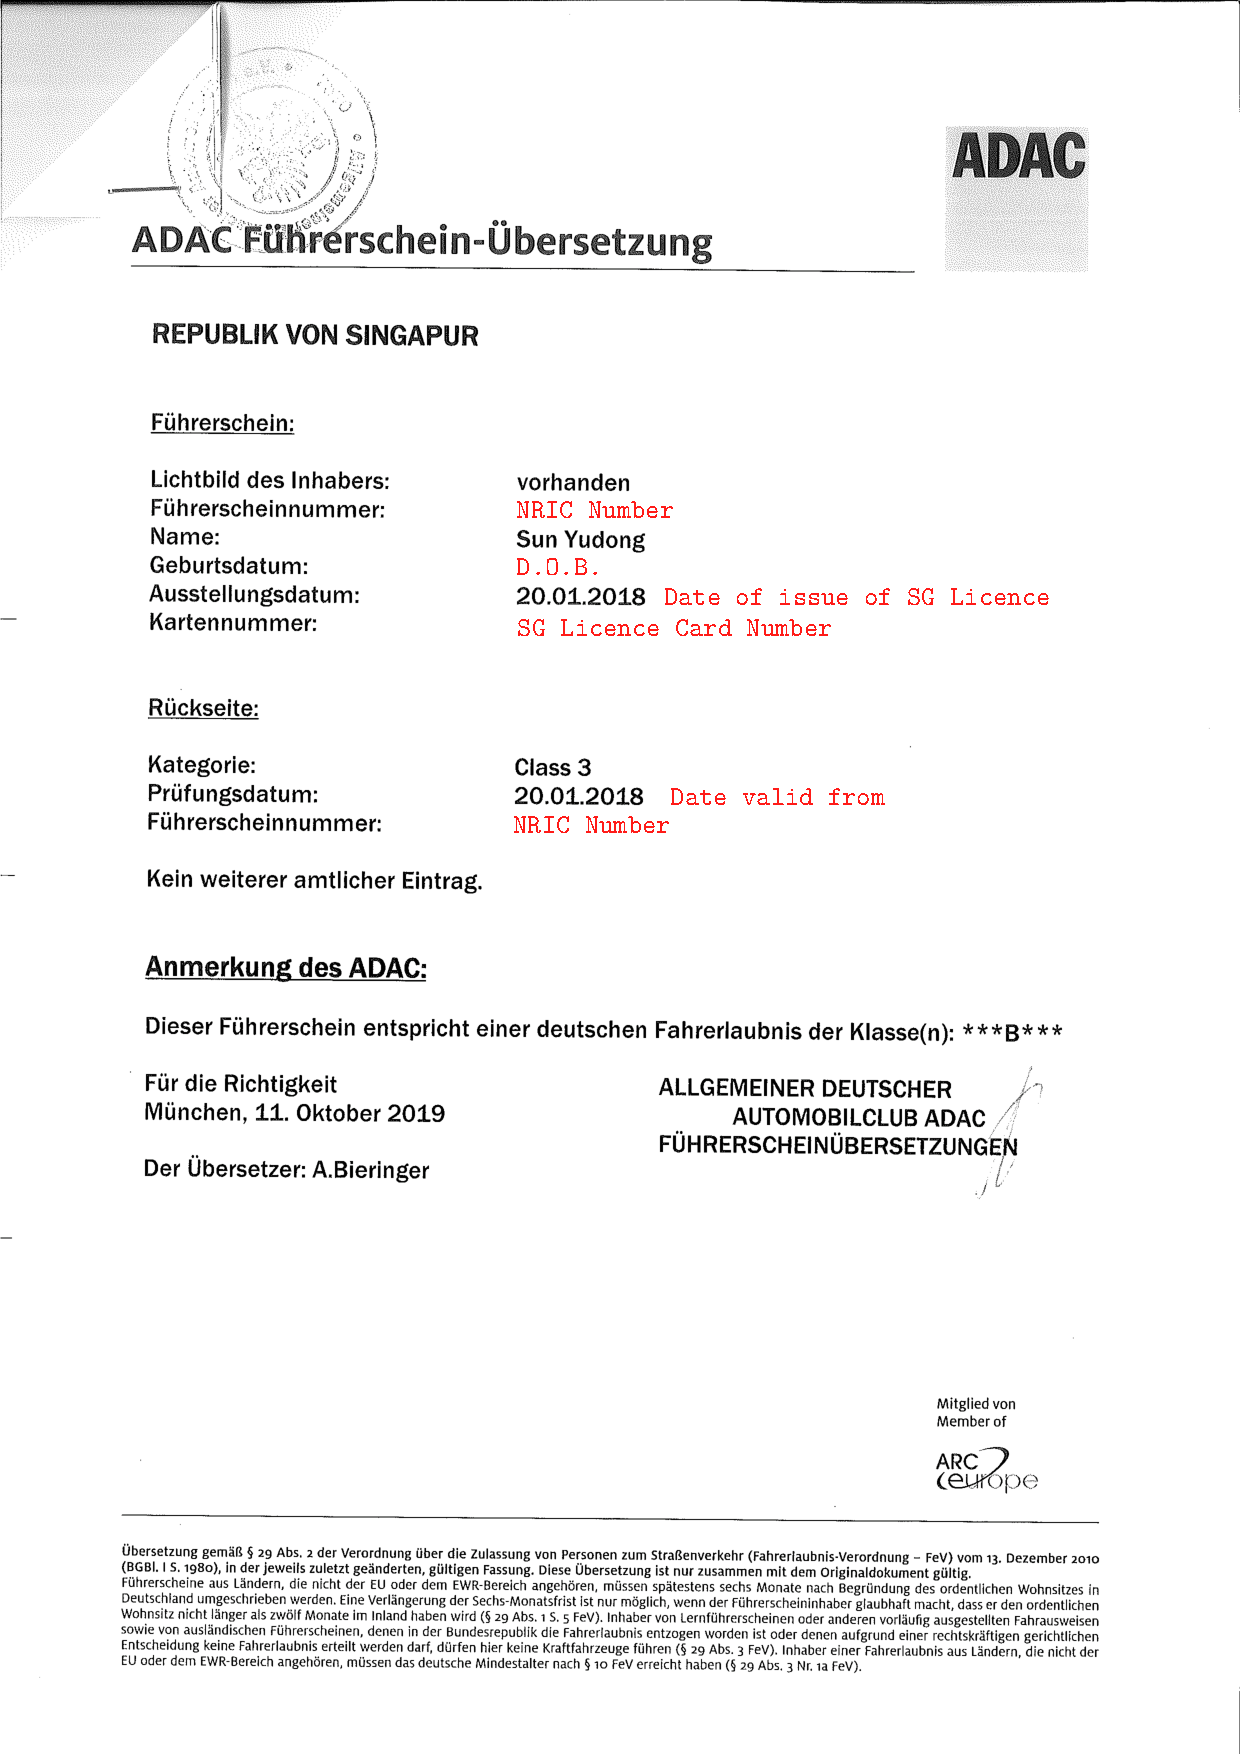
\includegraphics[width=0.6\textwidth]{ADAC.pdf}
        \caption{Translation. This will be submitted to KVR.}
        \label{fig:ADAC-Translation}
    \end{figure}
    
    This may be obtained from any ADAC branch office. The addresses may be obtained from the ADAC Website\footnote{\url{www.adac.de/der-adac/vor-ort/}}. There are multiple branches within Munich, you can go to any one of them. No appointment necessary.
    
    A simple translation takes about 30 minutes and can be done on the spot. For complicated cases (e.g. many complicated licence classes) it takes up to a day.  

\section{Applying for a conversion}
    \cost{35} \hspace{5mm} (Licence $\geq$ 2 Years)\par
    \cost{35.80} \hspace{5mm} (Licence $<$ 2 Years)
    
    \subsection{Documents Needed}
        \begin{enumerate}
            \item Valid Passport
            \item Valid physical Singapore Qualified Driving Licence
            \item 1 physical Biometric Photo (\SI{35}{\milli\meter} $\times$ \SI{45}{\milli\meter})
            \item Confirmation of \de{Anmeldung} for your current residence in Munich
            \item All confirmations of previous \de{Anmeldung} (should you have multiple) since your arrival in Germany
            \item ADAC Translation
            \item Additional Medical Documentation if you are converting a Class 4 or 5 Licence (Equivalent to Classes C and D)
        \end{enumerate}
        
        Class 3A licences may or may not be recognized. 
    
    \subsection{Appointment}
        Once you have the translation, you need to make an appointment online at \url{www.fuehrerscheine-muenchen.de}. Do note that you will have to personally go down for the appointment as a signature from you is required.
        
        \begin{enumerate}
            \item Select \de{Online-Terminvereinbarung}
            \item Under \de{Umschreibung eines ausländischen Führerscheins} select \de{Umschreibung eines ausländischen Führerscheins (kein EU/EWR-Führerschein) beantragen}
            \item Click \de{Weiter} to bring up available appointments
        \end{enumerate}
        
        At this point, you may find that there are little to no appointments available. Fret not, they do open some last minute same-day slots in the early mornings every day (read 6 am ish). So check back often to see if they have any new appointments. 
        
    \subsection{In person process}
        Once you book your appointment, bring all your documents down to:
        
        \begin{center}
            Kreisverwaltungsreferat (KVR) \\
            Hauptabteilung II Fahrzeugzulassungs- und Fahrerlaubnisbehörde \\
            Garmischer Str. 19-21 \\
            81377 München \\
            
            Tel: 089 233-96090
        \end{center}
        
        There will be a security standing outside the main office to guide you. 
        
        As part of the application, you will need to submit your original Singapore QDL. This is so that the local police can check for its validity. You will get your Singapore QDL back after the check is completed.
        
        They will also issue you the following document to prove that your licence is with the authorities. You may use that document in place of your licence should you wish to drive within this period (so long as it is within the aforementioned 6 months).
        
        \begin{figure}[H]
            \centering
            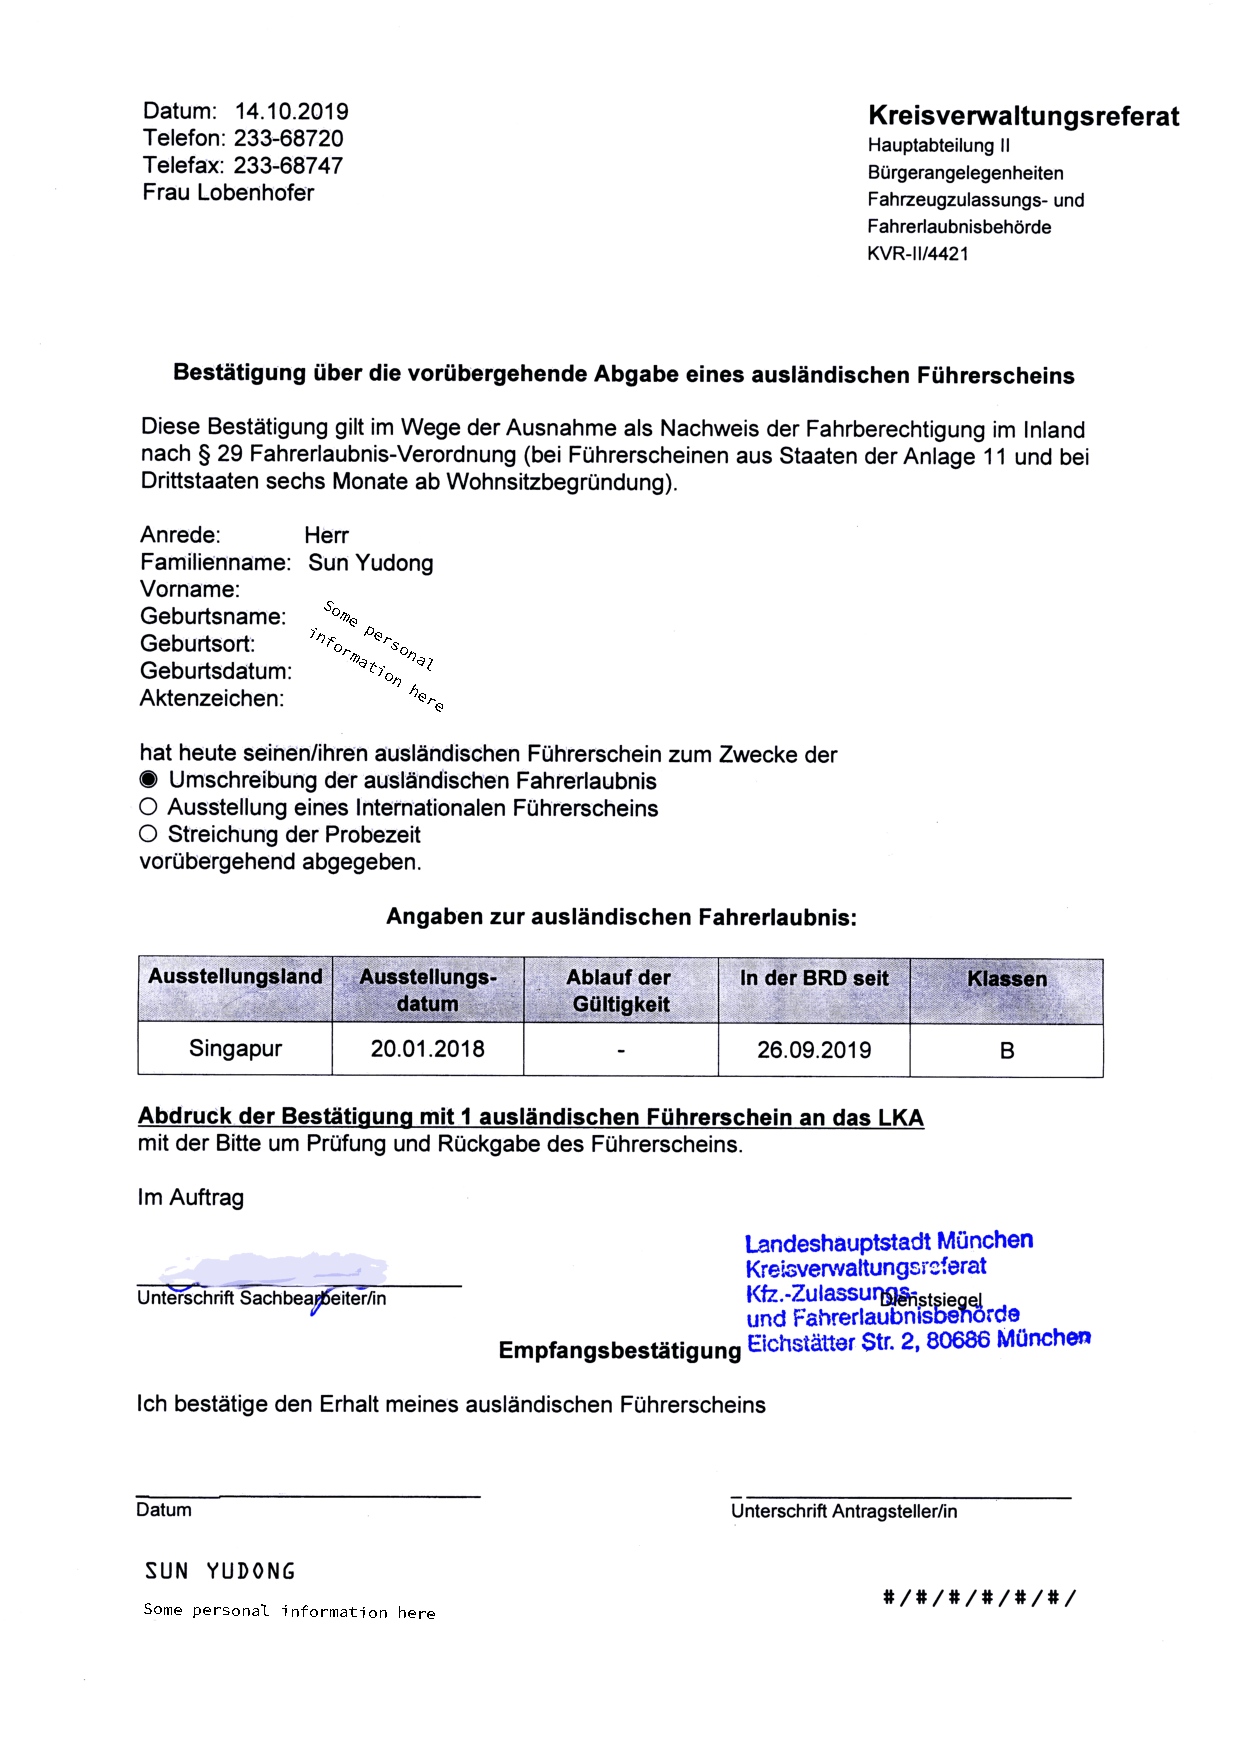
\includegraphics[width=0.63\textwidth]{collection.pdf}
            \caption{Collection Form}
            \label{fig:collection}
        \end{figure}
        
        In Germany, the \de{Probezeit} or Probation period is 2 years. As the author's date of application (2019-10-14) is still within the probation period (from 2018-01-20), it costed $35.80$ \euro~instead of just $35.00$ \euro.
        
        After you have complete this step, all you have to do is wait for them to notify you via snail mail when the German Driving Licence is ready for your collection.
    
    \subsection{Roadblocks} \label{subsec:roadblocks}
        Unfortunately, it may not be so straightforward. After waiting for 2 months, the author did not receive anything from the KVR. If you encounter something similar, it is crucial to personally go down to their office to inquire about it. 
        
        In the author's case, the physical licence was not ordered after the police verification was completed and it resulted in a very long delay. The office ordered it immediately and issued a provisional licence (a red piece of paper, \de{Vorläufigen Nachweis der Fahrerlaubnis}). This document is a valid Driving Licence within Germany only. 

        Waiting for the physical licence took a further 2 weeks after the inquiry due to the holiday season (hence the 10 to 12 weeks).
        
\section{Collection of the Converted Licence}
    
\section{Additional Resources}
    You may find more information at the following links. They might be in German:
    \begin{itemize}
        \item \url{www.muenchen.de/rathaus/Stadtverwaltung/Kreisverwaltungsreferat/Verkehr/Fuehrerschein.html}
    \end{itemize}
    
    There are also a few infosheets attached at the end of this document for more detailed information. 
    
    All documents are provided on an as-is basis, and serve merely as a guide. These documents do not have any authority. When in doubt, always check with the KVR office themselves.
    
\section{Contributions}
    This document and relevant files are synced with \href{https://github.com/sunjerry019/SGDEDrivingLicenceGuide}{github.com/sunjerry019/SGDEDrivingLicenceGuide}. Feel free to make PRs, raise issues and contact me. All contributions are welcome.

\pagebreak 
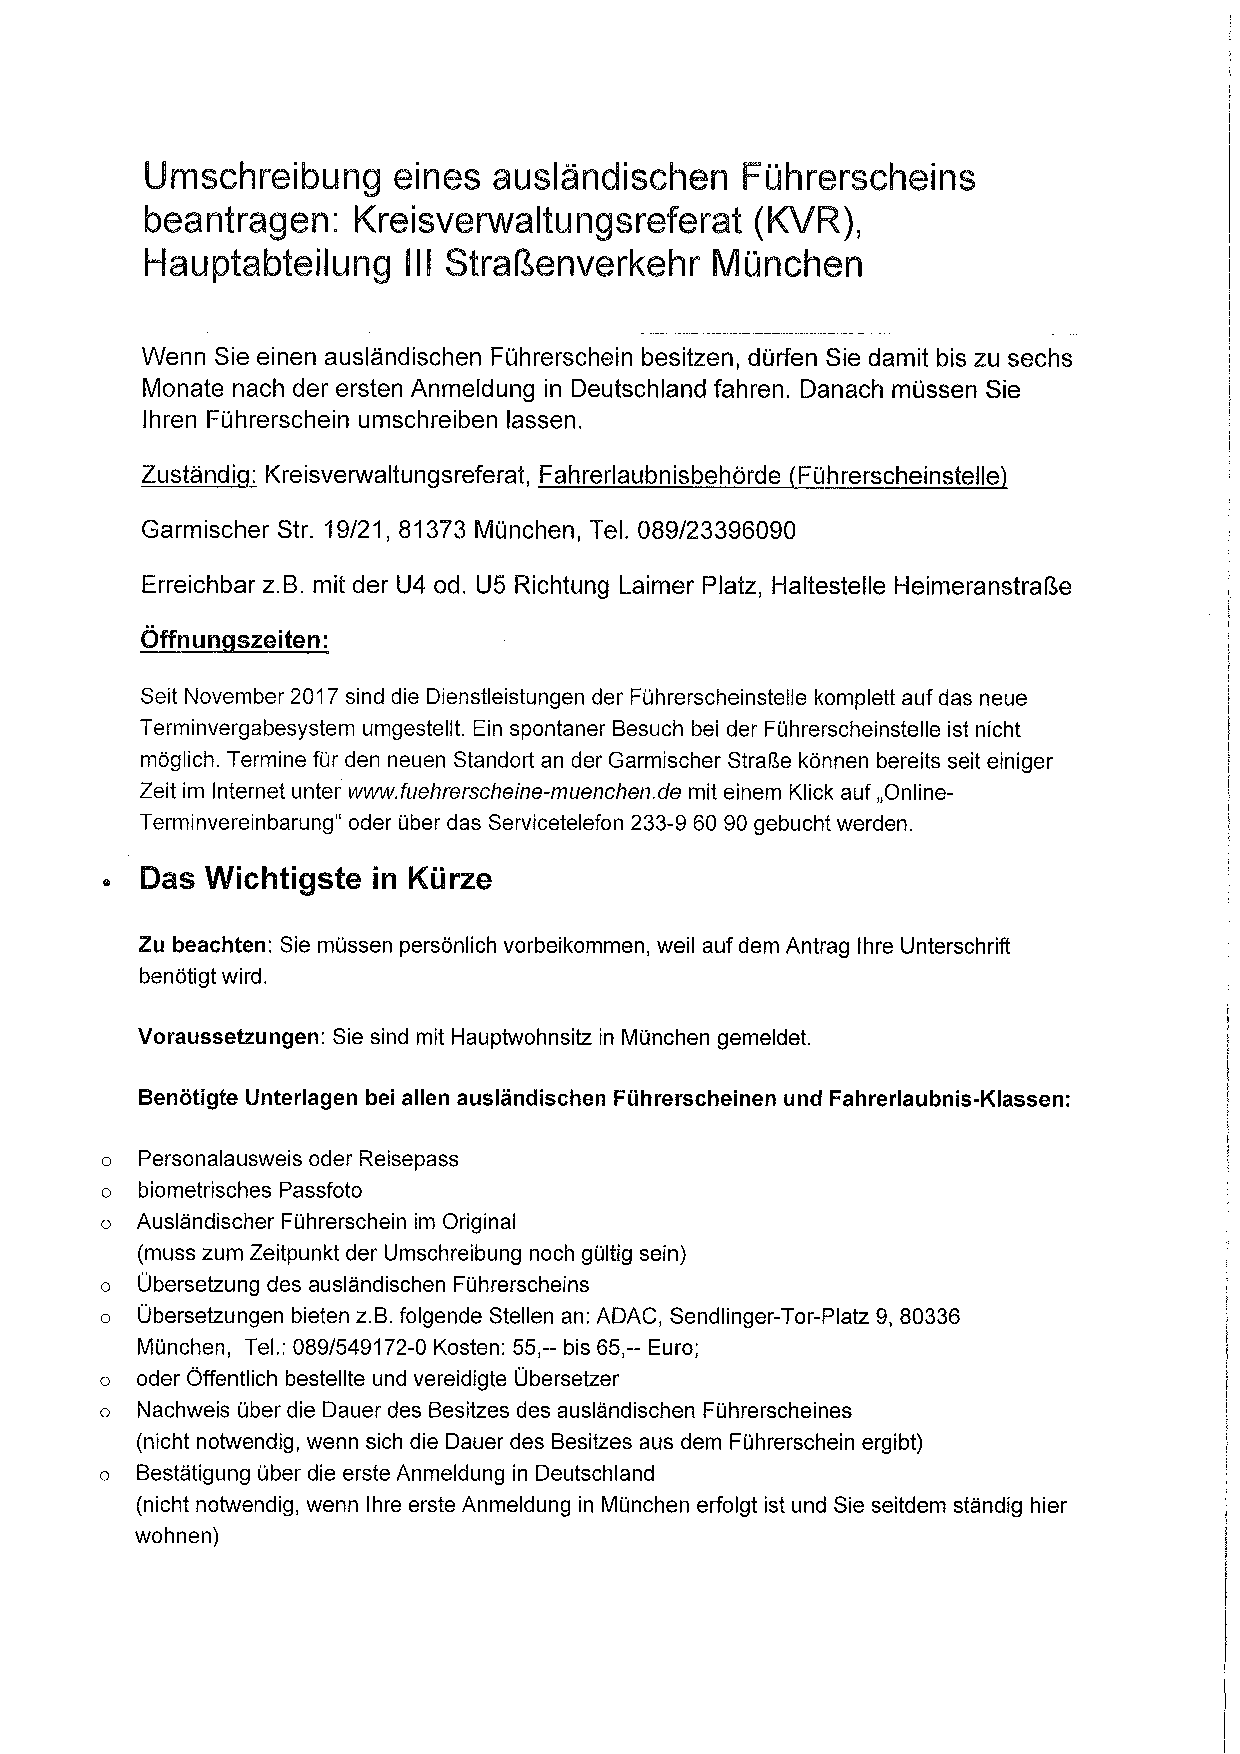
\includepdf[]{attachments/ADAC-Infosheet.pdf}
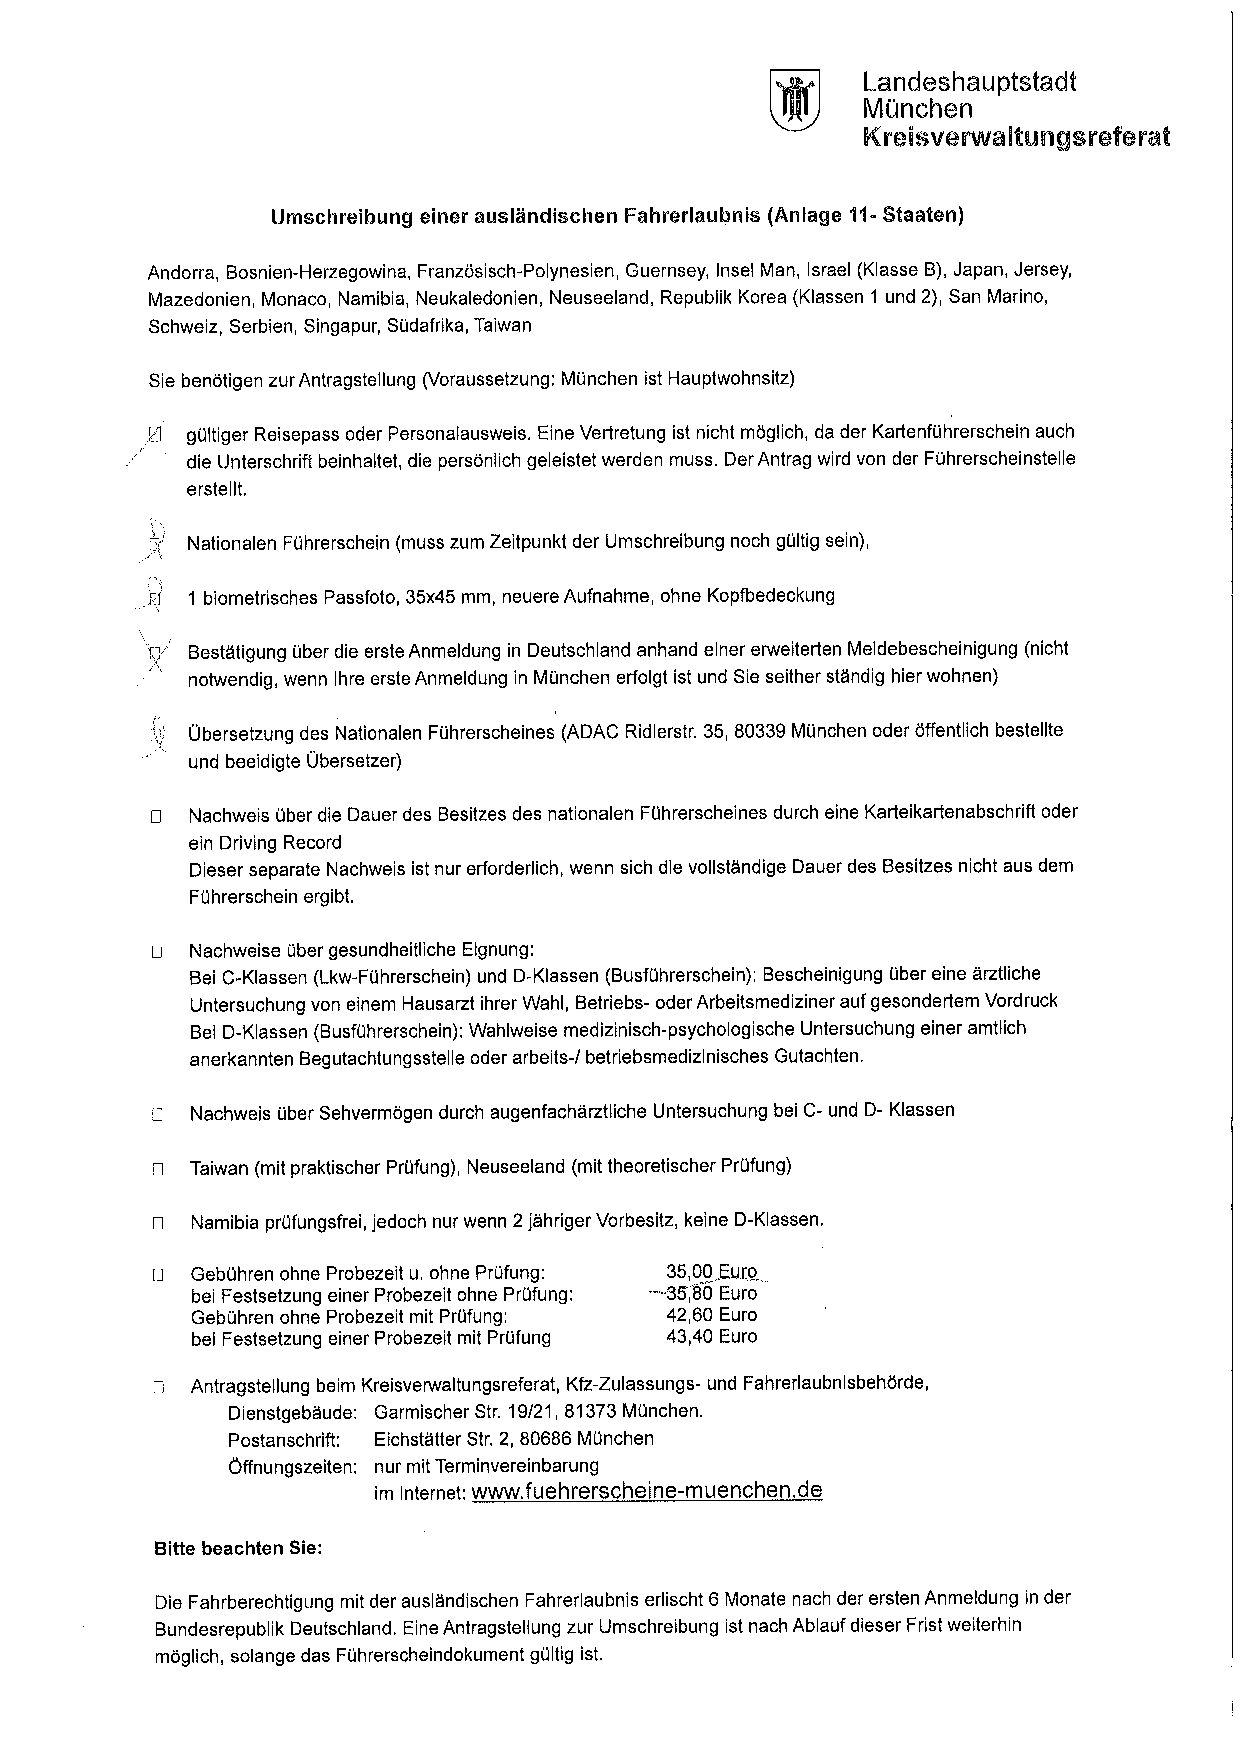
\includepdf[]{attachments/KVR-Infosheet.pdf}
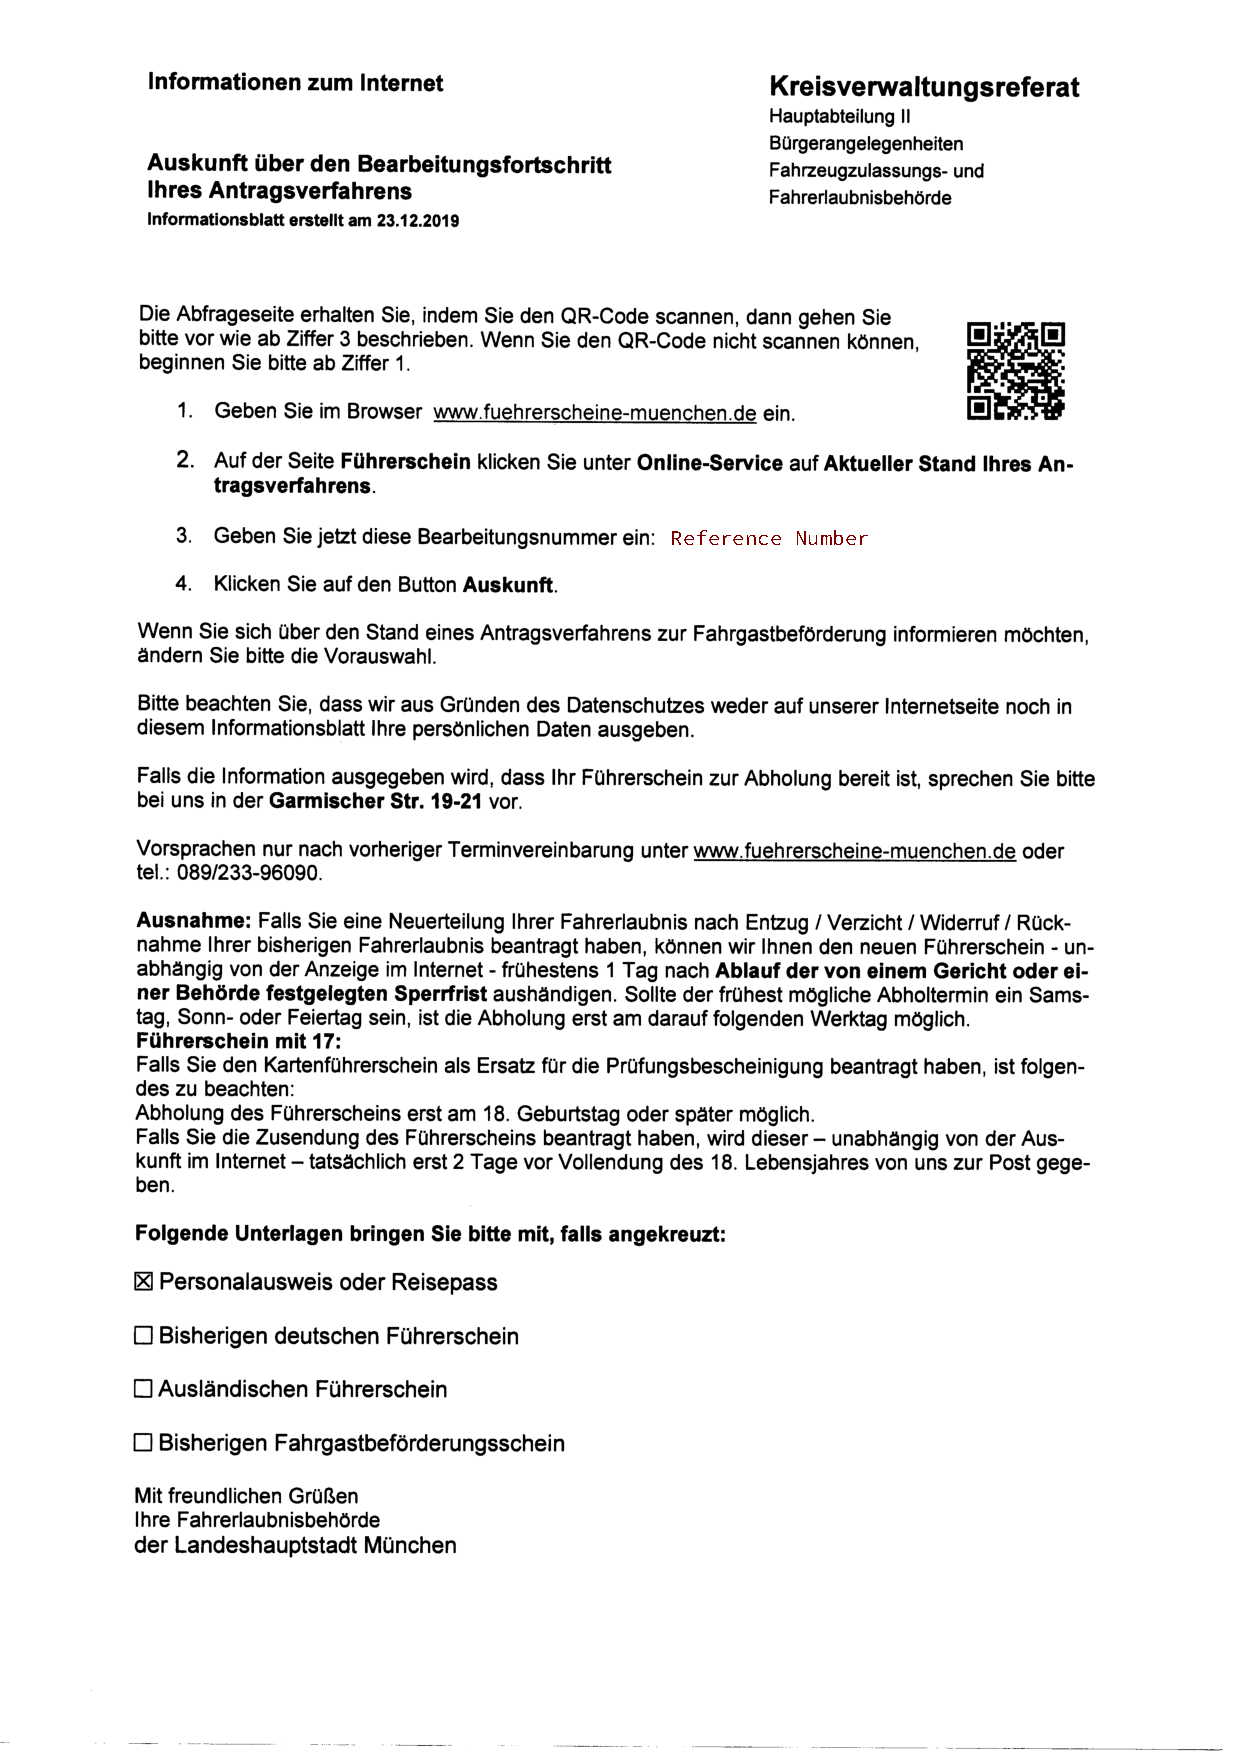
\includepdf[]{attachments/status.pdf}

\end{document}
